\section*{Part 4 [75 points]}

\begin{enumerate}
\itemsep 2em
    
    \item \textbf{[19 points]} Use the following \texttt{mcperf} command to vary QPS from 5K to 125K in order to answer the following questions: 
    \begin{Verbatim}[fontsize=\small]
$ ./mcperf -s INTERNAL_MEMCACHED_IP --loadonly 
$ ./mcperf -s INTERNAL_MEMCACHED_IP -a INTERNAL_AGENT_IP  \
           --noload -T 8 -C 8 -D 4 -Q 1000 -c 8 -t 2 \ 
           --scan 5000:125000:10000
    \end{Verbatim}

    a) [8 points] How does memcached performance vary with the number of threads ($T$) and number of cores ($C$) allocated to the job? In a single graph, plot the 95th percentile latency (y-axis) vs. achieved QPS (x-axis) of memcached (running alone, with no other jobs collocated on the server) for the following configurations (one line each):
    \begin{itemize}
        \item Memcached with $T$=1 thread, $C$=1 core
        \item Memcached with $T$=1 thread, $C$=2 cores
        \item Memcached with $T$=1 thread, $C$=3 cores
        \item Memcached with $T$=2 threads, $C$=1 core
        \item Memcached with $T$=2 threads, $C$=2 cores
        \item Memcached with $T$=2 threads, $C$=3 cores
        \item Memcached with $T$=3 thread, $C$=1 cores
        \item Memcached with $T$=3 thread, $C$=2 cores
        \item Memcached with $T$=3 threads, $C$=3 cores
    \end{itemize}
    
    Label the axes in your plot. State how many runs you averaged across (we recommend three runs) and include error bars. The readability of your plot will be part of your grade.
    
    \textbf{Plots:} % Place your plots here.
    \begin{figure}[H]
        \centering
        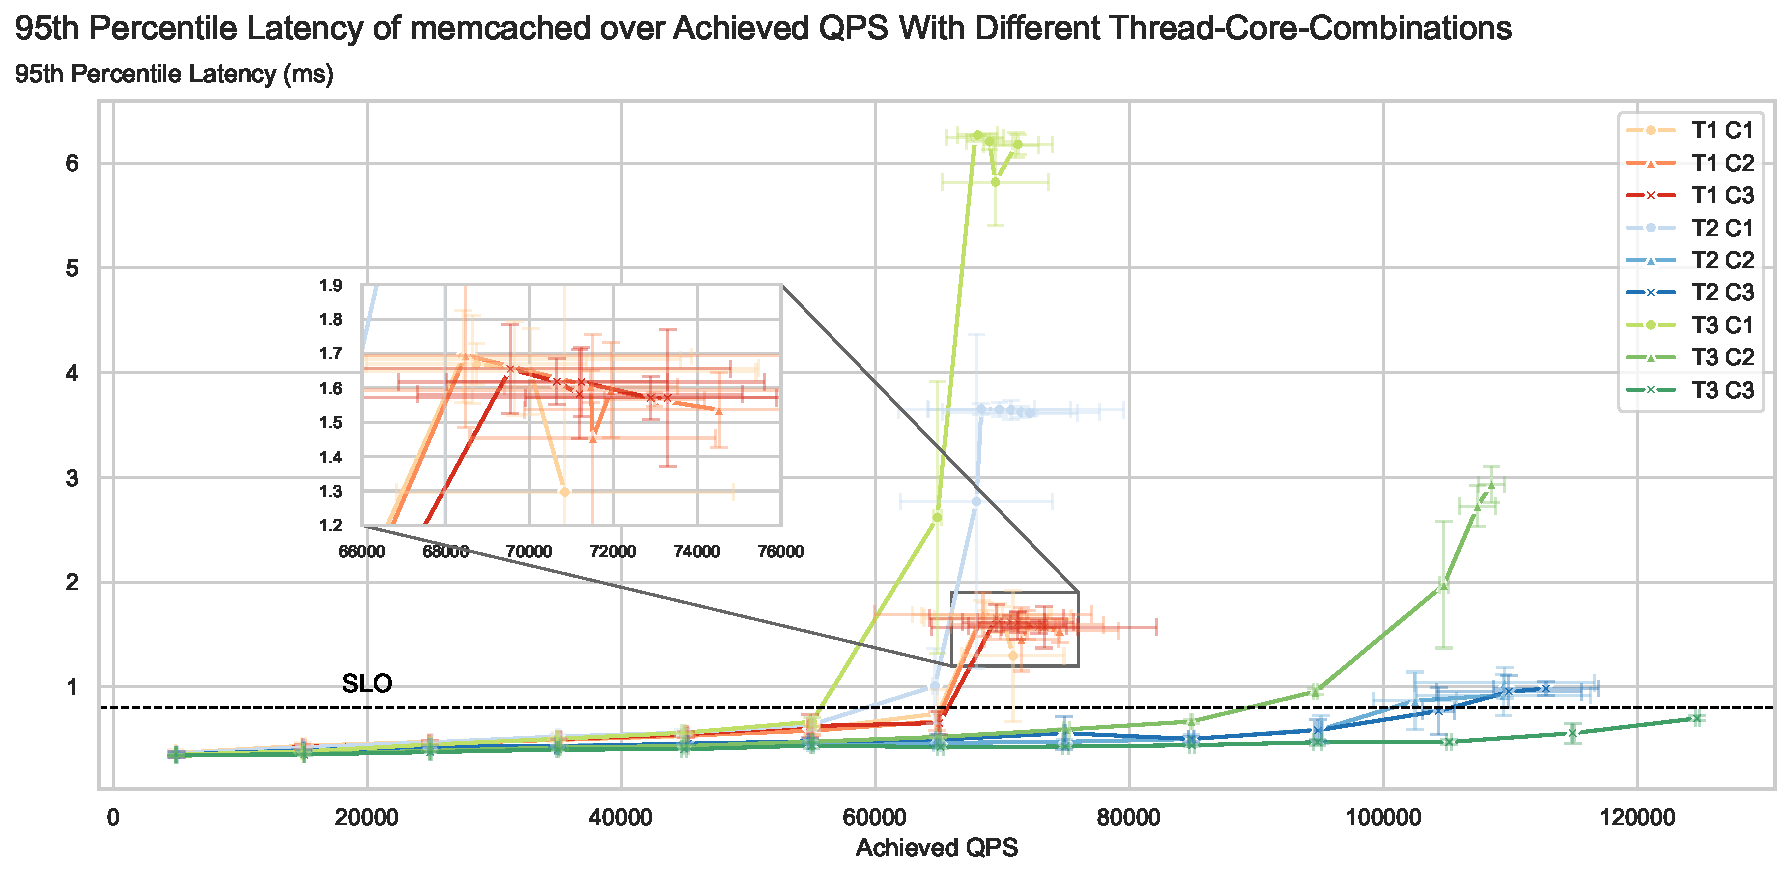
\includegraphics[width=1\linewidth]{report/figures/part4_plot1.pdf}
        \caption{Memcached 95th percentile latency in milliseconds over the achieved QPS, for 1 to 3 threads and for each thread 1 to 3 cores. The black line represents the SLO of $0.8ms$.}
        \label{fig:part4_plot1}
    \end{figure}

    
    What do you conclude from the results in your plot? Summarize in 2-3 brief sentences how memcached performance varies with the number of threads and cores and how this relates to the target QPS.
    
    \textbf{Summary:} % Place your solution here.
    Using one thread, the number of cores neihter changes the achieved QPS nor the 95th percentile latency. When increasing the number of threads, but not of cores, the achieved QPS stays the same, with a maximum of around $50\%$ of the target QPS, but the latency goes up for more threads, and when the number of cores is the same to the number of threads, neither the achieved QPS, nor the 95th percentile latency will improve when further increasing the number of threads, and when increasing the number of threads and the number of cores, the performanc increases for both, and the achieved QPS almost reaches target QPS with 3 threads and 3 cores. The higher the target QPS gets, the more the 95th percentile latency increases.
    \\
    
    b) [2 points] To support the highest load in the trace (around 125K QPS) without violating the 0.8ms latency SLO, how many memcached threads ($T$) and CPU cores ($C$) will you need?
    
    \textbf{Answer:} % Place your solution here.
    With the highest QPS trace of 125K, the only combination that achieves to stay below the SLO of $0.8$ms is with 3 threads and 3 cores. Therefore, $T=3$ and $C=3$ would be needed.
    \\
    
    c) [1 point] Assume you can change the number of cores allocated to memcached dynamically as the QPS varies from 5K to 125K, but the number of threads is fixed when you launch the memcached job. How many memcached threads ($T$) do you propose to use to guarantee the 0.8ms 95th percentile latency SLO while the load varies between 5K to 125K QPS?
    
    \textbf{Answer:} % Place your solution here.
    As the only combination that achieves the to stay below the SLO of $0.8$ms for the 95th percentile latency of memcached for 125K QPS is $T=3$ and $C=3$, it is necessary to choose $T=3$, that in the worst case of 125K QPS, the number of cores can be increased so SLO is guaranteed.
    \\
    
    d) [8 points] Run memcached with the number of threads $T$ that you proposed in (c) and measure performance with $C=1$, $C=2$ and $C=3$. Use the aforementioned \texttt{mcperf} command to sweep QPS from 5K to 125K.

    Measure the CPU utilization on the memcached server at each load time step. Plot the performance of memcached using 1-core ($C=1$), 2 cores ($C=2$) and 3 ($C=3$) in \textbf{three separate graphs}, for $C=1$, $C=2$ and $C=3$, respectively. In each graph, plot achieved QPS on the x-axis, ranging from 0 to 125K. In each graph, use two y-axes. Plot the 95th percentile latency on the left y-axis. Draw a dotted horizontal line at the 0.8ms latency SLO. Plot the CPU utilization (ranging from 0\% to 100\% for $C=1$, 200\% for $C=2$ and 300\% for $C=3$) on the right y-axis. For simplicity, we do not require error bars for these plots. 
    
    \textbf{Plots:} % Place your plots here.
    \begin{figure}[H]
        \centering
        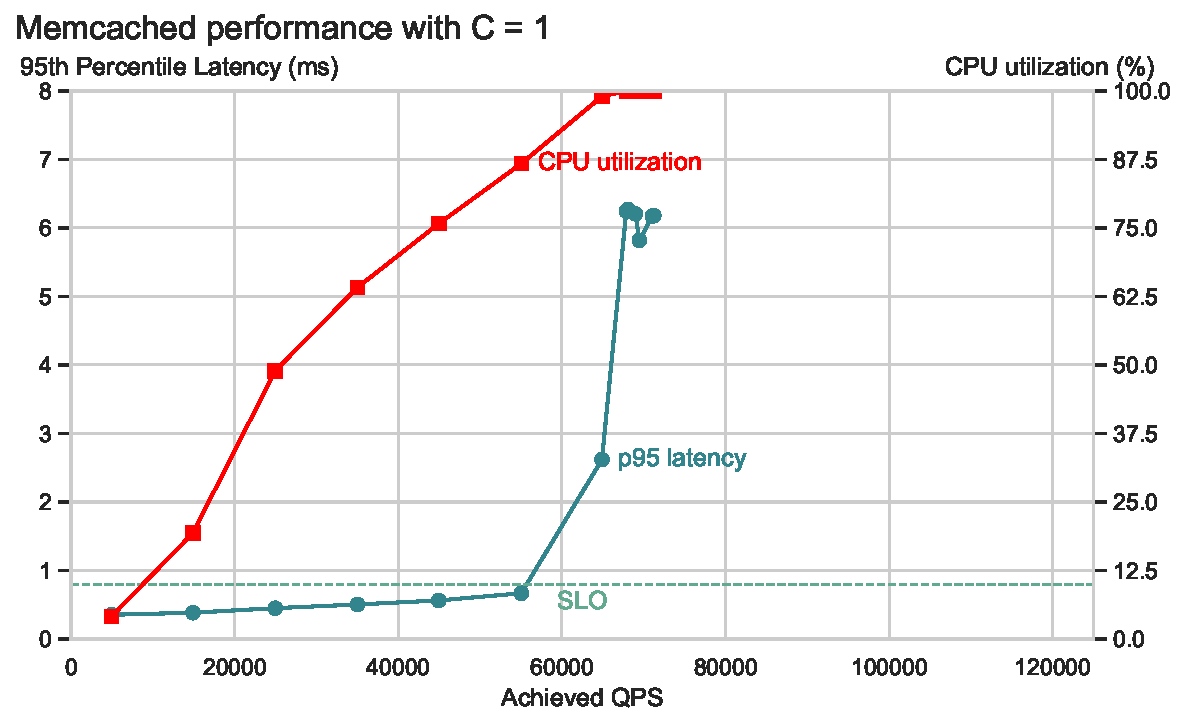
\includegraphics[width=0.8\linewidth]{report/figures/part4_plotC_1.pdf}
        \caption{Memcached 95th percentile latency on the left axis in blue and CPU utilization on the right axis in read over achieved QPS, when running memcached with 3 threads on 1 core.}
        \label{fig:part4_plotC_1}
    \end{figure}

    \begin{figure}[H]
        \centering
        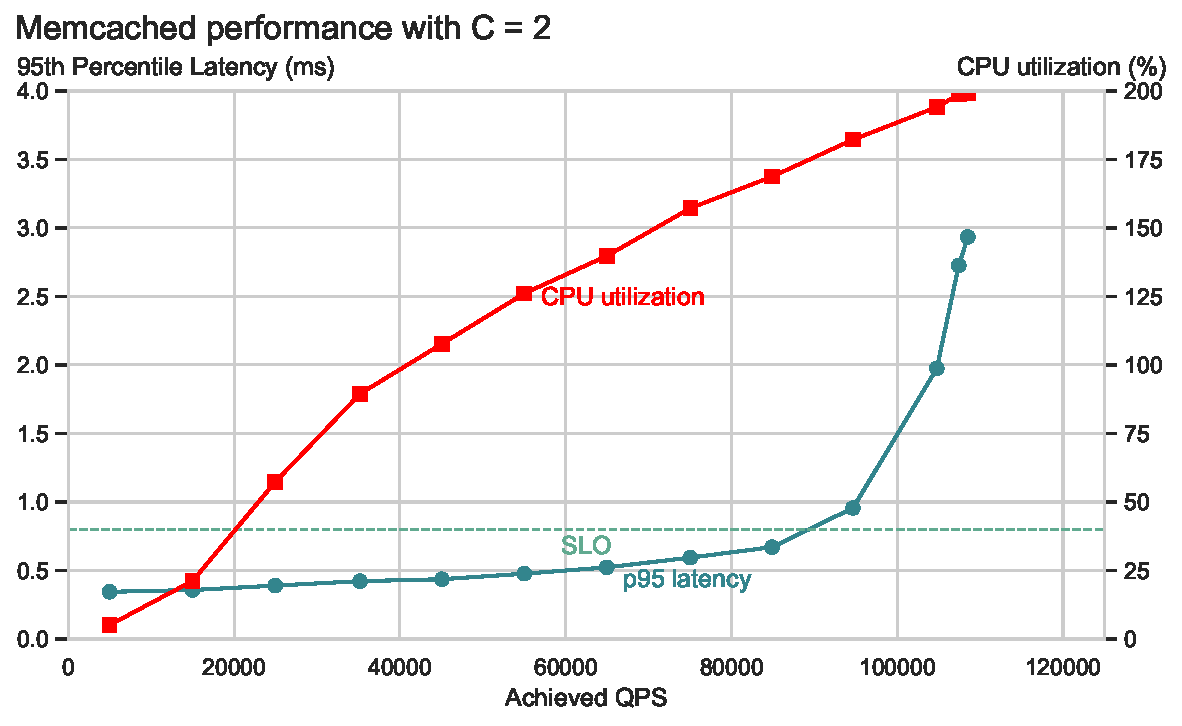
\includegraphics[width=0.8\linewidth]{report/figures/part4_plotC_2.pdf}
        \caption{Memcached 95th percentile latency on the left axis in blue and CPU utilization on the right axis in read over achieved QPS, when running memcached with 3 threads on 2 cores.}
        \label{fig:part4_plotC_2}
    \end{figure}

    \begin{figure}[H]
        \centering
        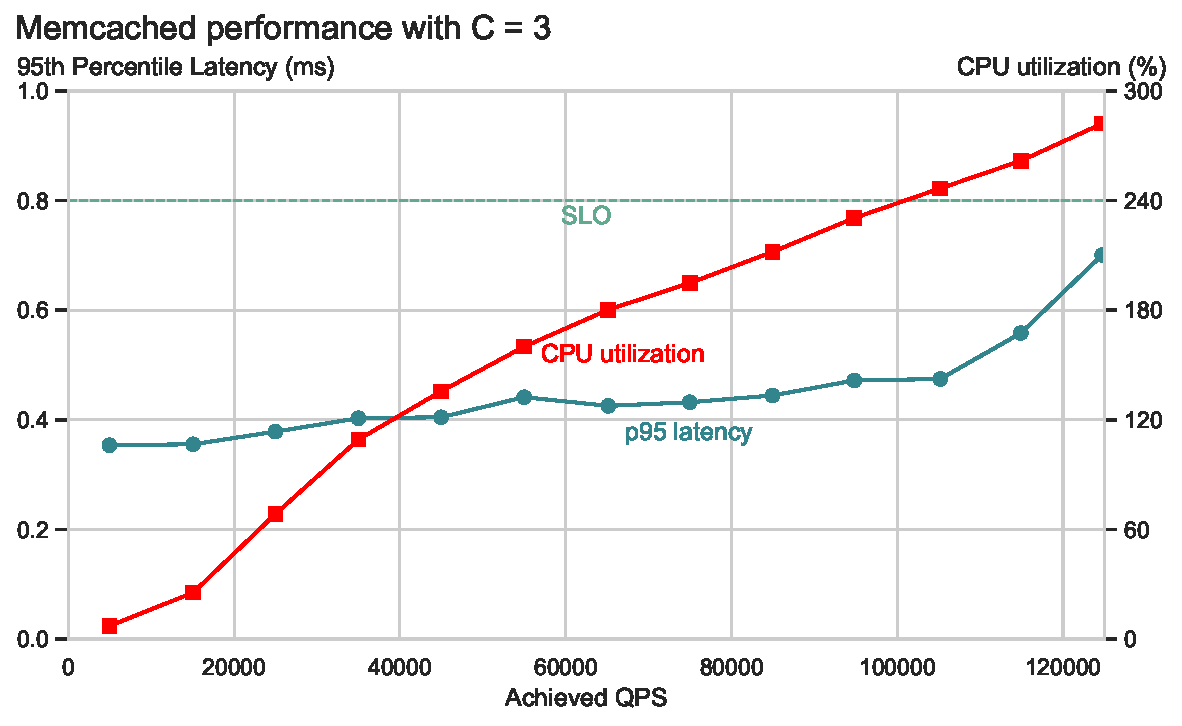
\includegraphics[width=0.8\linewidth]{report/figures/part4_plotC_3.pdf}
        \caption{Memcached 95th percentile latency on the left axis in blue and CPU utilization on the right axis in read over achieved QPS, when running memcached with 3 threads on 3 cores.}
        \label{fig:part4_plotC_3}
    \end{figure}

    
    \item \textbf{[17 points]} You are now given a dynamic load trace for memcached, which varies QPS randomly between 5K and 110K in 15 second time intervals. Use the following command to run this trace: 
        \begin{Verbatim}[fontsize=\small]
$ ./mcperf -s INTERNAL_MEMCACHED_IP --loadonly 
$ ./mcperf -s INTERNAL_MEMCACHED_IP -a INTERNAL_AGENT_IP \ 
           --noload -T 8 -C 8 -D 4 -Q 1000 -c 8 -t 1800 \ 
           --qps_interval 15 --qps_min 5000 --qps_max 110000
\end{Verbatim}
    
    Note that you can also specify a random seed in this command using the \texttt{--qps\_seed} flag. 

    For this and the next questions, feel free to reduce the mcperf measurement duration (\texttt{-t} parameter, now fixed to 30 minutes) as long as you have at the end at least 1 minute of memcached running alone.
    \\
    
    Design and implement a controller to schedule memcached and the benchmarks (batch jobs) on the 4-core VM. The goal of your scheduling policy is to successfully complete all batch jobs as soon as possible without violating the 0.8ms 95th percentile latency for memcached. \textbf{Your controller should not assume prior knowledge of the dynamic load trace. You should design your policy to work well regardless of the random seed.} The batch jobs need to use the native dataset, i.e., provide the option \texttt{-i native} when running them. Also make sure to check that all the batch jobs complete successfully and do not crash. Note that batch jobs may fail if given insufficient resources. \\
    
    Describe how you designed and implemented your scheduling policy. Include the source code of your controller in the zip file you submit. 

    \begin{itemize}
        \item Brief overview of the scheduling policy (max 10 lines):
        
    \textbf{Answer:} % Place your solution here.
    The controller always reserves core 0 for memcached and dynamically shares cores 1--3 between memcached and batch jobs, where memcached gets at most 3 cores at any given moment. Every 0.3\,s, it reads \texttt{/proc/stat} to compute per-core CPU utilization and applies asymmetric thresholds to scale memcached up (at 80\% by one core – by two cores at 90\% spikes) or down (at $<$70\%). Phase 1 runs splash2x jobs (radix, barnes) concurrently. Phase 2 runs the remaining PARSEC jobs sequentially with all available cores; this removes resource contention. The controller pre-creates all containers at startup for instant launches, and avoids the slow Python Docker API as much as possible by handling PIDs directly.
    \\
     
    \item How do you decide how many cores to dynamically assign to memcached? Why?
    
    \textbf{Answer:}
    The controller monitors aggregate CPU utilization across all cores assigned to memcached (core 0 plus leftover cores among cores 1--3). If utilization exceeds $90\% \cdot N_\text{cores}$, it gives memcached 2 additional cores; if it exceeds $80\% \cdot N_\text{cores}$, it gives 1 additional core. Memcached only returns a core to the batch jobs when \textit{post-drop} utilization would be below $70\%$, i.e current utilization less than $70\% \cdot (N_\text{cores} - 1)$, meaning memcached could sustain its load with one fewer core. The threshold asymmetry prevents oscillation and thrashing – ensures utilization stays between $70\%$ -- $80\%$ per core.

    Cores are allocated \textit{stickily}, e.g. suppose memcached runs on core 0, barnes runs on cores 1-2, and radix runs on core 3; if the controller determines memcached needs one more core, memcached will run on cores {0,3}; there is never unnecessary shuffling of cores.
    \\

    \item How do you decide how many cores to assign each batch job? Why?

    \textbf{Answer:}
    The general principle is: 1. avoid contention, and 2. rather let the OS schedule threads on fewer cores and ensure temporal locality (stickiness), over constantly trying to fit jobs with fewer threads onto a changing number of cores, constantly flushing the cache.
    
    The only reason, that barnes and radix deviate from this principle is, due to the power-of-2 restriction on splash2x jobs' number of threads.
    \begin{itemize}
        \item \colored{barnes}: Up to 2 cores. 

        \item \colored{blackscholes}: Up to 3 cores.

        \item \colored{canneal}: Up to 3 cores.

        \item \colored{freqmine}: Up to 3 cores. 

        \item \colored{radix}: 1 core.

        \item \colored{streamcluster}: Up to 3 cores. 

        \item \colored{vips}: Up to 3 cores.
        \\
    \end{itemize}


    \item How many threads do you use for each of the batch job? Why?
    
    \textbf{Answer:}
    In accordance with the aformentioned principle, PARSEC jobs have 3 threads; barnes' and radix's number of threads ensure they roughly terminate simulataneously.
    \begin{itemize}
        \item \colored{barnes}: 2 threads, ensuring its runtime roughly matches up with radix on 1 thread.

        \item \colored{blackscholes}: 3 threads.

        \item \colored{canneal}: 3 threads.

        \item \colored{freqmine}: 3 threads.

        \item \colored{radix}: 1 thread.

        \item \colored{streamcluster}: 3 threads.

        \item \colored{vips}: 3 threads.
        \\
    \end{itemize}
      
    \item Which jobs run concurrently / are collocated and on which cores? Why?

    \textbf{Answer:}
    All jobs' sets of cores are always disjoint. Phase 1 runs radix (1 core) and barnes (up to 2 cores) concurrently, and their exact cores may change over time, due to, how the controller maximizes stickiness. Once one of the two jobs finishes, the controller starts blackscholes alongside the remaining job when possible. These splash2x jobs are short and are fairly complimentary (radix memory-bound, barnes compute-bound), so co-scheduling has low contention. Phase 2 runs all PARSEC jobs sequentially (one at a time on a dynamically changing subset of cores 1--3). As mentioned, if fewer cores are available, the controller relies on the OS scheduler to multiplex between threads.
    \\
    
    \item In which order did you run the batch jobs? Why?

    \textbf{Order} (to be sorted): % Sort them 
    \{\colored{radix}, \colored{barnes}\} $\to$ \colored{blackscholes} $\to$ \colored{canneal} $\to$ \colored{freqmine} $\to$ \colored{streamcluster} $\to$ \colored{vips}
    
    \textbf{Why:}
    Radix and barnes start concurrently, because they are splash2x workloads and require power-of-two thread counts. Allocating 1 and 2 threads respectively and running them concurrently is preferable over over-allocating 4 threads to each. Finishing them early simplifies sequential scheduling afterwards. Blackscholes starts as soon as either one finishes, overlapping with the remaining unfinished job. The Phase 2 PARSEC jobs (canneal, freqmine, streamcluster, vips) run sequentially on 3 threads to minimize contention.
    \\

\item How does your policy differ from the policy in Part 3? Why?

\textbf{Answer:} % Place your solution here.
The policy in Part 3 runs in a completely different context with 12 cores instead of 4 cores available. In Part 3, thanks to a consistently light load on memcached, one can generously colocate the least scalable jobs on the same 4-core node as memcached, maximizing parallelism on the 8-core node with minimal contention by running jobs sequentially. A shared principle seen in Part 3 and Part 4 is, to minimize resource contention, by running jobs sequentially.
\\

\item How did you implement your policy? e.g., docker cpu-set updates, taskset updates for memcached, pausing/unpausing containers, etc.

\textbf{Answer:} % Place your solution here.
The controller calls \texttt{taskset -a -cp} to dynamically pin memcached's to a set of CPUs (covering all kernel threads). For batch jobs, it pre-creates containers via Docker and starts them when scheduled. Core updates write directly to the cgroup v2 file for minimal latency. When a job must temporarily yield all cores to memcached, the controller calls \texttt{container.pause()} / \texttt{container.unpause()}. CPU utilization comes from reading \texttt{/proc/stat} every 0.3\,s and computing per-core busy-time deltas. The Python Docker API is slow and blocking; the controller successfully avoids interacting with it, for detecting finished jobs and updating cores; only starting, pausing and unpausing involve the API.
\\

\item Describe the design choices, ideas and trade-offs you took into account while creating your scheduler (\underline{if not already mentioned above}). Describe how your policy (and its performance) compares to another policy that you experimented with (in particular to the second-best policy that you designed).

\textbf{Answer:} % Put your solution here
The polling interval length trades responsiveness for measurement noise; shorter intervals produce noisy readings and oscillation, longer intervals risk missing load spikes.

Asymmetric thresholds ($>80\%$/$90\%$ scale up, $<70\%$ scale down) prevent hysteresis. The tradeoff is between stability and optimal utilization.

Pre-creating containers eliminates Docker image pull and creation latency from the critical path.

Pinning the controller to a core other than core 0, which always belongs to memcached, ensures, that memcached tends to run uninterfered.
\\
\end{itemize}

\item \textbf{[23 points]} Run the following \texttt{mcperf} memcached dynamic load trace: 
    
\begin{Verbatim}[fontsize=\small]
$ ./mcperf -s INTERNAL_MEMCACHED_IP --loadonly 
$ ./mcperf -s INTERNAL_MEMCACHED_IP -a INTERNAL_AGENT_IP \ 
           --noload -T 8 -C 8 -D 4 -Q 1000 -c 8 -t 1800 \ 
           --qps_interval 15 --qps_min 5000 --qps_max 110000 \ 
           --qps_seed 2345
\end{Verbatim}
    
    
    Measure memcached and batch job performance when using your scheduling policy to launch workloads and dynamically adjust container resource allocations. Run this workflow 3 separate times. For each run, measure the execution time of each batch job, as well as the latency outputs of memcached. For each batch application, compute the mean and standard deviation of the execution time \footnote{Here, you should only consider the runtime, excluding time spans during which the container is paused.} across three runs. Compute the mean and standard deviation of the total time to complete all jobs - the makespan of all jobs. Fill in the table below.  Also, compute the SLO violation ratio for memcached for each of the three runs; the number of data points with 95th percentile latency $>$ 0.8ms, as a fraction of the total number of datapoints. The SLO violation ratio should be calculated during the time from when the first batch-job-container starts running to when the last batch-job-container stops running. \\
    
    \begin{table}[ht]
        \centering
        \begin{tabular}{ |c|c|c|c|c|} 
            \hline
            job name & mean time [s] & std [s] \\ \hline \hline
            \coloredcell{barnes}          & 90.94 & 5.00 \\  \hline
            \coloredcell{blackscholes}    & 80.23 & 1.69 \\  \hline
            \coloredcell{canneal}         & 149.18 & 26.34 \\  \hline
            \coloredcell{freqmine}        & 350.33 & 20.83 \\  \hline
            \coloredcell{radix}           & 45.75 & 1.93 \\  \hline
            \coloredcell{streamcluster}   & 333.17 & 1.01 \\  \hline
            \coloredcell{vips}            & 78.54 & 19.72 \\  \hline
            total time      & 1107.16 & 22.65 \\  \hline
        \end{tabular}
    \end{table}

    \textbf{Answer:}
    On average, our policy had a runtime of $1107.16$ seconds ($\approx 18.5$ minutes) with a standard deviation of $22.65$ seconds. The jobs vips, canneal and freqmine had much higher standard deviations than the other jobs, resulting in the increase of the standrad deviation of the total time. The longest time to finish took streamcluster with an average of $333.17$ seconds, but a low standard deviation, and therefore a stable runtime over the different runs of our policy.

    The 95th percentile latency constantly stayed below $0.6$ ms across all runs. With an SLO of $0.8$ ms, we were meeting the SLO in all three runs. Thus, we had $0\%$ SLO violations.

    \[\text{SLO violaition ration} = \frac{\text{\#datapoints with p95} > 0.8 \text{ms}}{\text{\#p95 datapoints}} = \frac{0}{\text{\#p95 datapoints}} =  0\%\]
    

    Include three plots -- one for each of the three runs -- with the following information: The x-axis should be the time from execution start to end. Use three subplots that share the same x-axis. The first should clearly indicate for each core what job it is running at all time (e.g. using colored boxes). Use the colors proposed in this template (you can find them in \texttt{main.text}). If you pause/unpause jobs as part of your scheduling policy this should also be clearly visible. The second subplot should include two y-axis where the left one shows the current QPS and the right one should include the achieved p95 latency. Finally, the third subplot should plot the cpu utilization of each core separately. The readability of your plot will be part of awarded points.
    %Include six plots -- two plots for each of the three runs -- with the following information. Label the plots as 1A, 1B, 2A, 2B, 3A, and 3B where the number indicates the run and the letter indicates the type of plot (A or B), which we describe below. In all plots, time will be on the x-axis and you should annotate the x-axis to indicate which benchmark (batch) application starts executing at which time. If you pause/unpause any workloads as part of your policy, you should also indicate the timestamps at which jobs are paused and unpaused. All the plots will have have two y-axes. The right y-axis will be QPS. For Plots A, the left y-axis will be the 95th percentile latency. For Plots B, the left y-axis will be the number of CPU cores that your controller allocates to memcached. For the plot, use the colors proposed in this template (you can find them in \texttt{main.tex}).

   \textbf{Plots:} % Place your plots here.
   \begin{figure}[H]
       \centering
       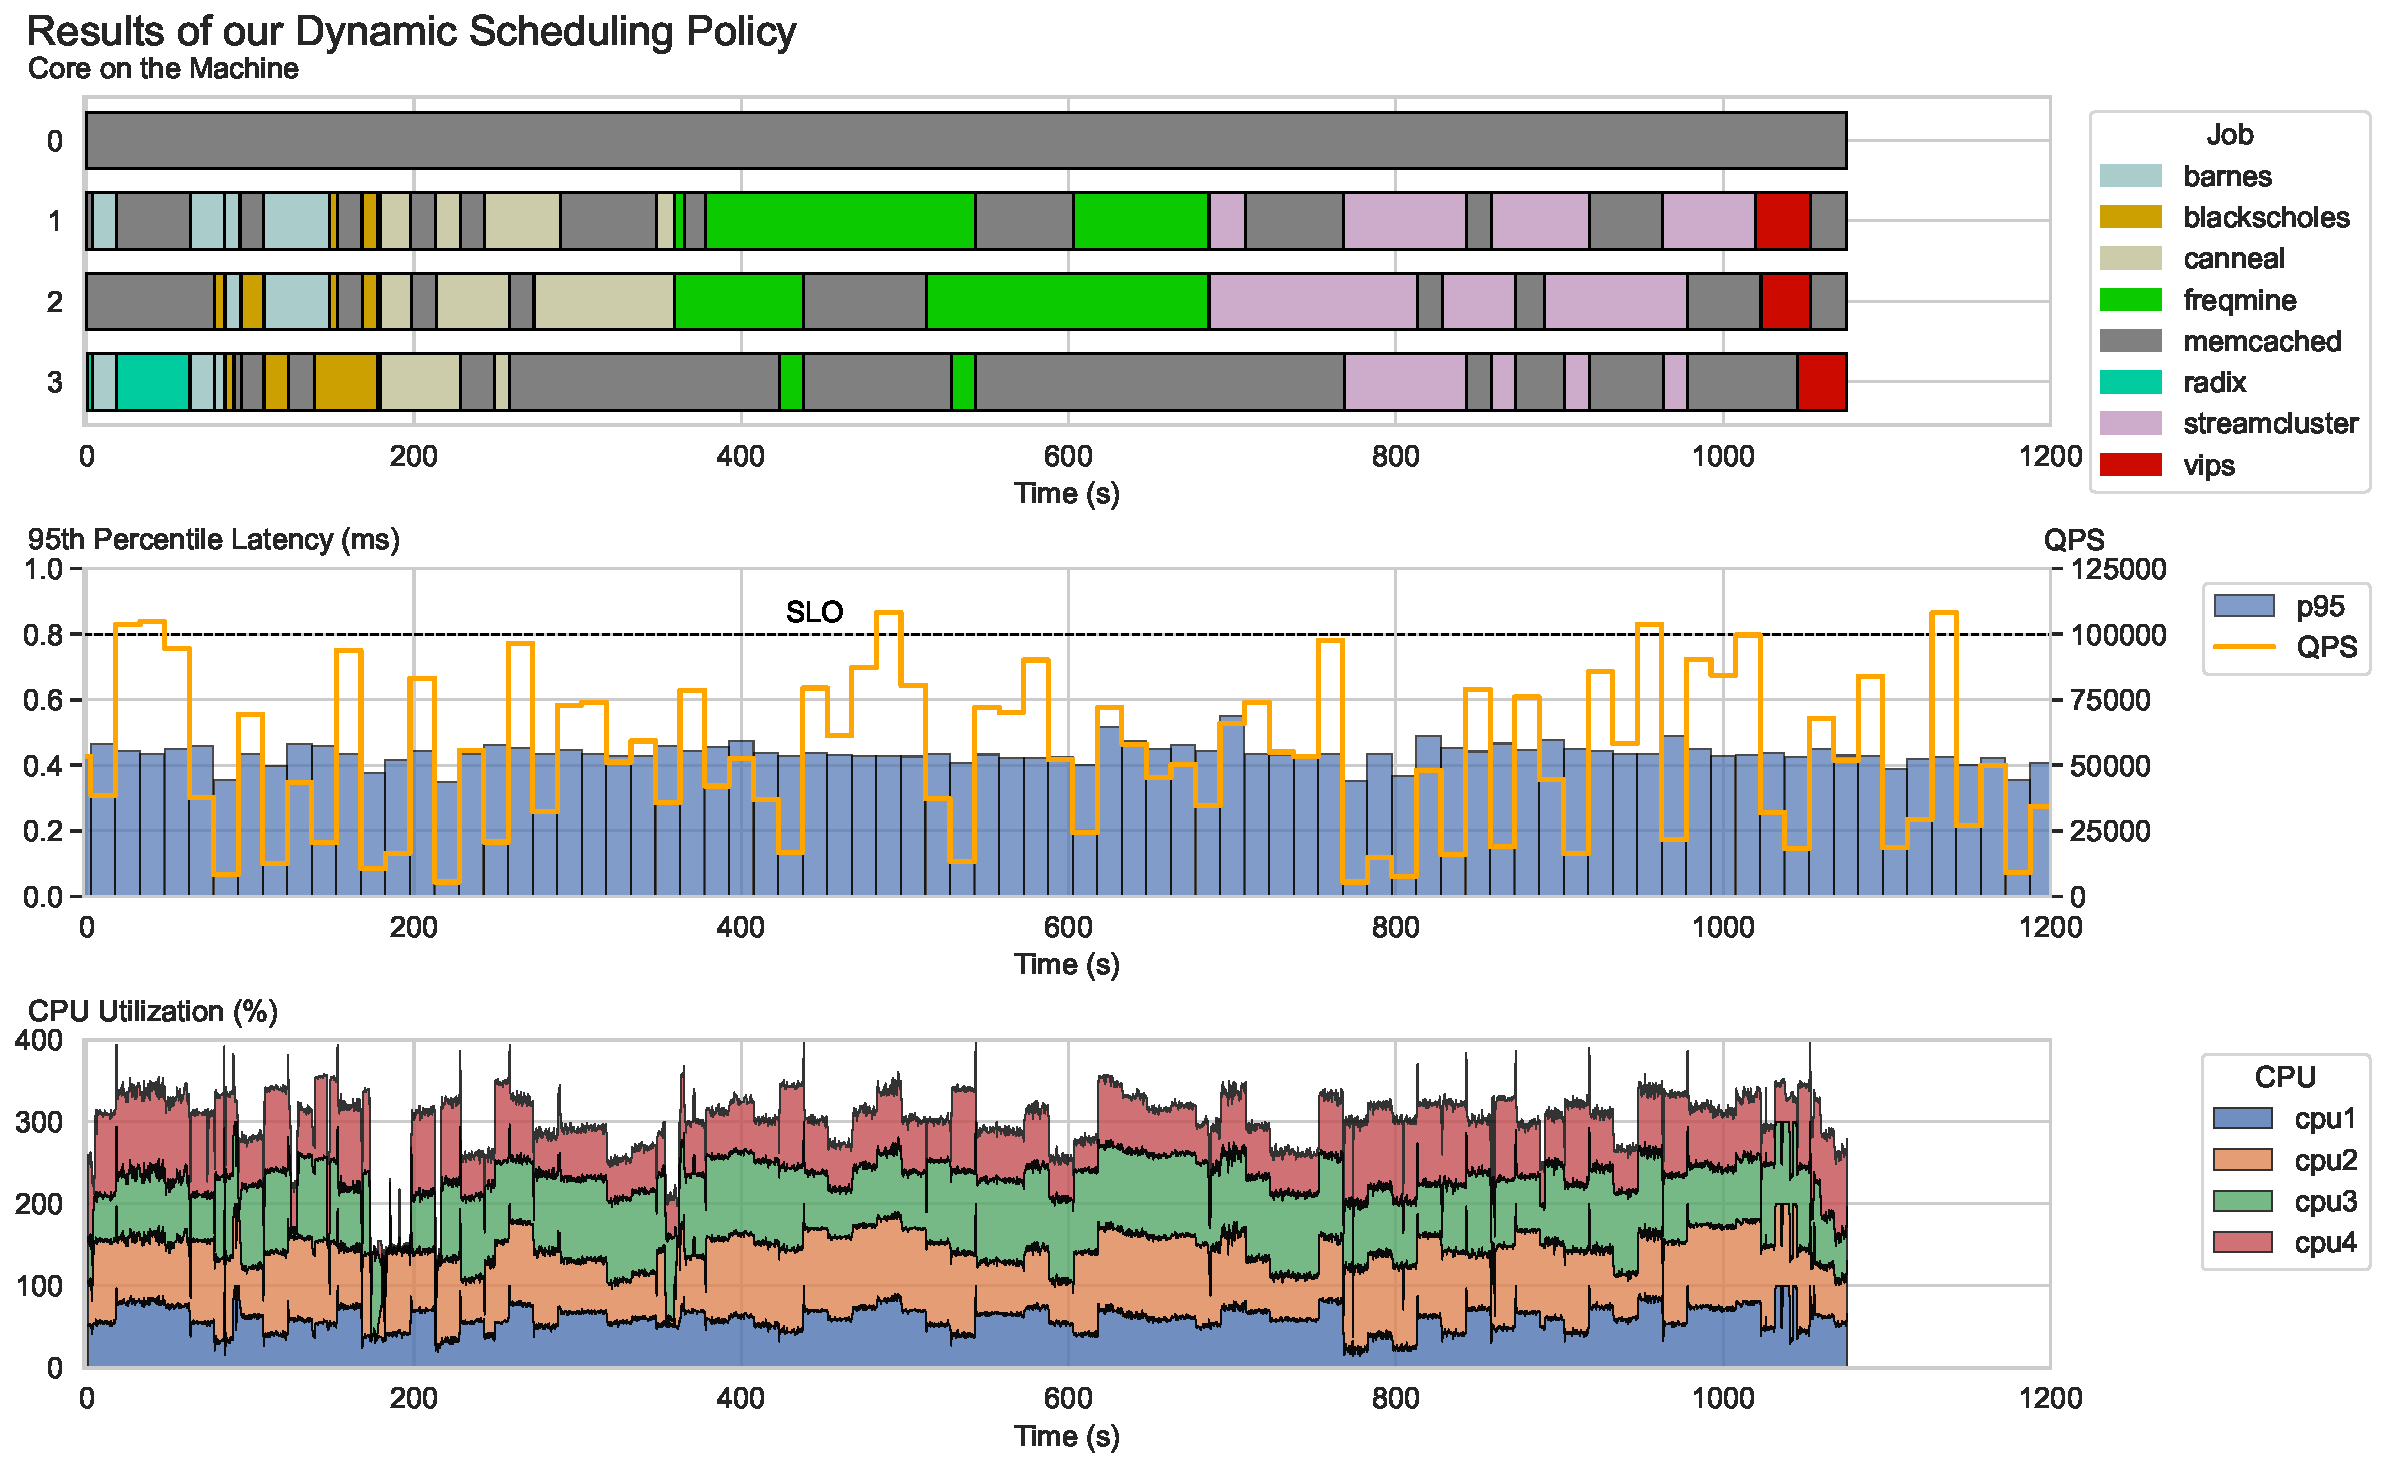
\includegraphics[width=1\linewidth]{report/figures/part4_q3_1.pdf}
       \caption{First run of our dynamic scheduling policy, showing on the first plot the scheduling of the jobs over the cores over time, on the second plot the 95th percentile latency (blue bars) with the SLO of $0.8 ms$ as a black line, and achieved QPS (orange line) over time, and on the third plot the CPU utilization of the cores. Running all jobs took $\approx 1076$ seconds ($\approx 17.9$ minutes), and resulted in $0\%$ violations of the SLO.}
       \label{fig:part4_q3_1}
   \end{figure}

   \begin{figure}[H]
       \centering
       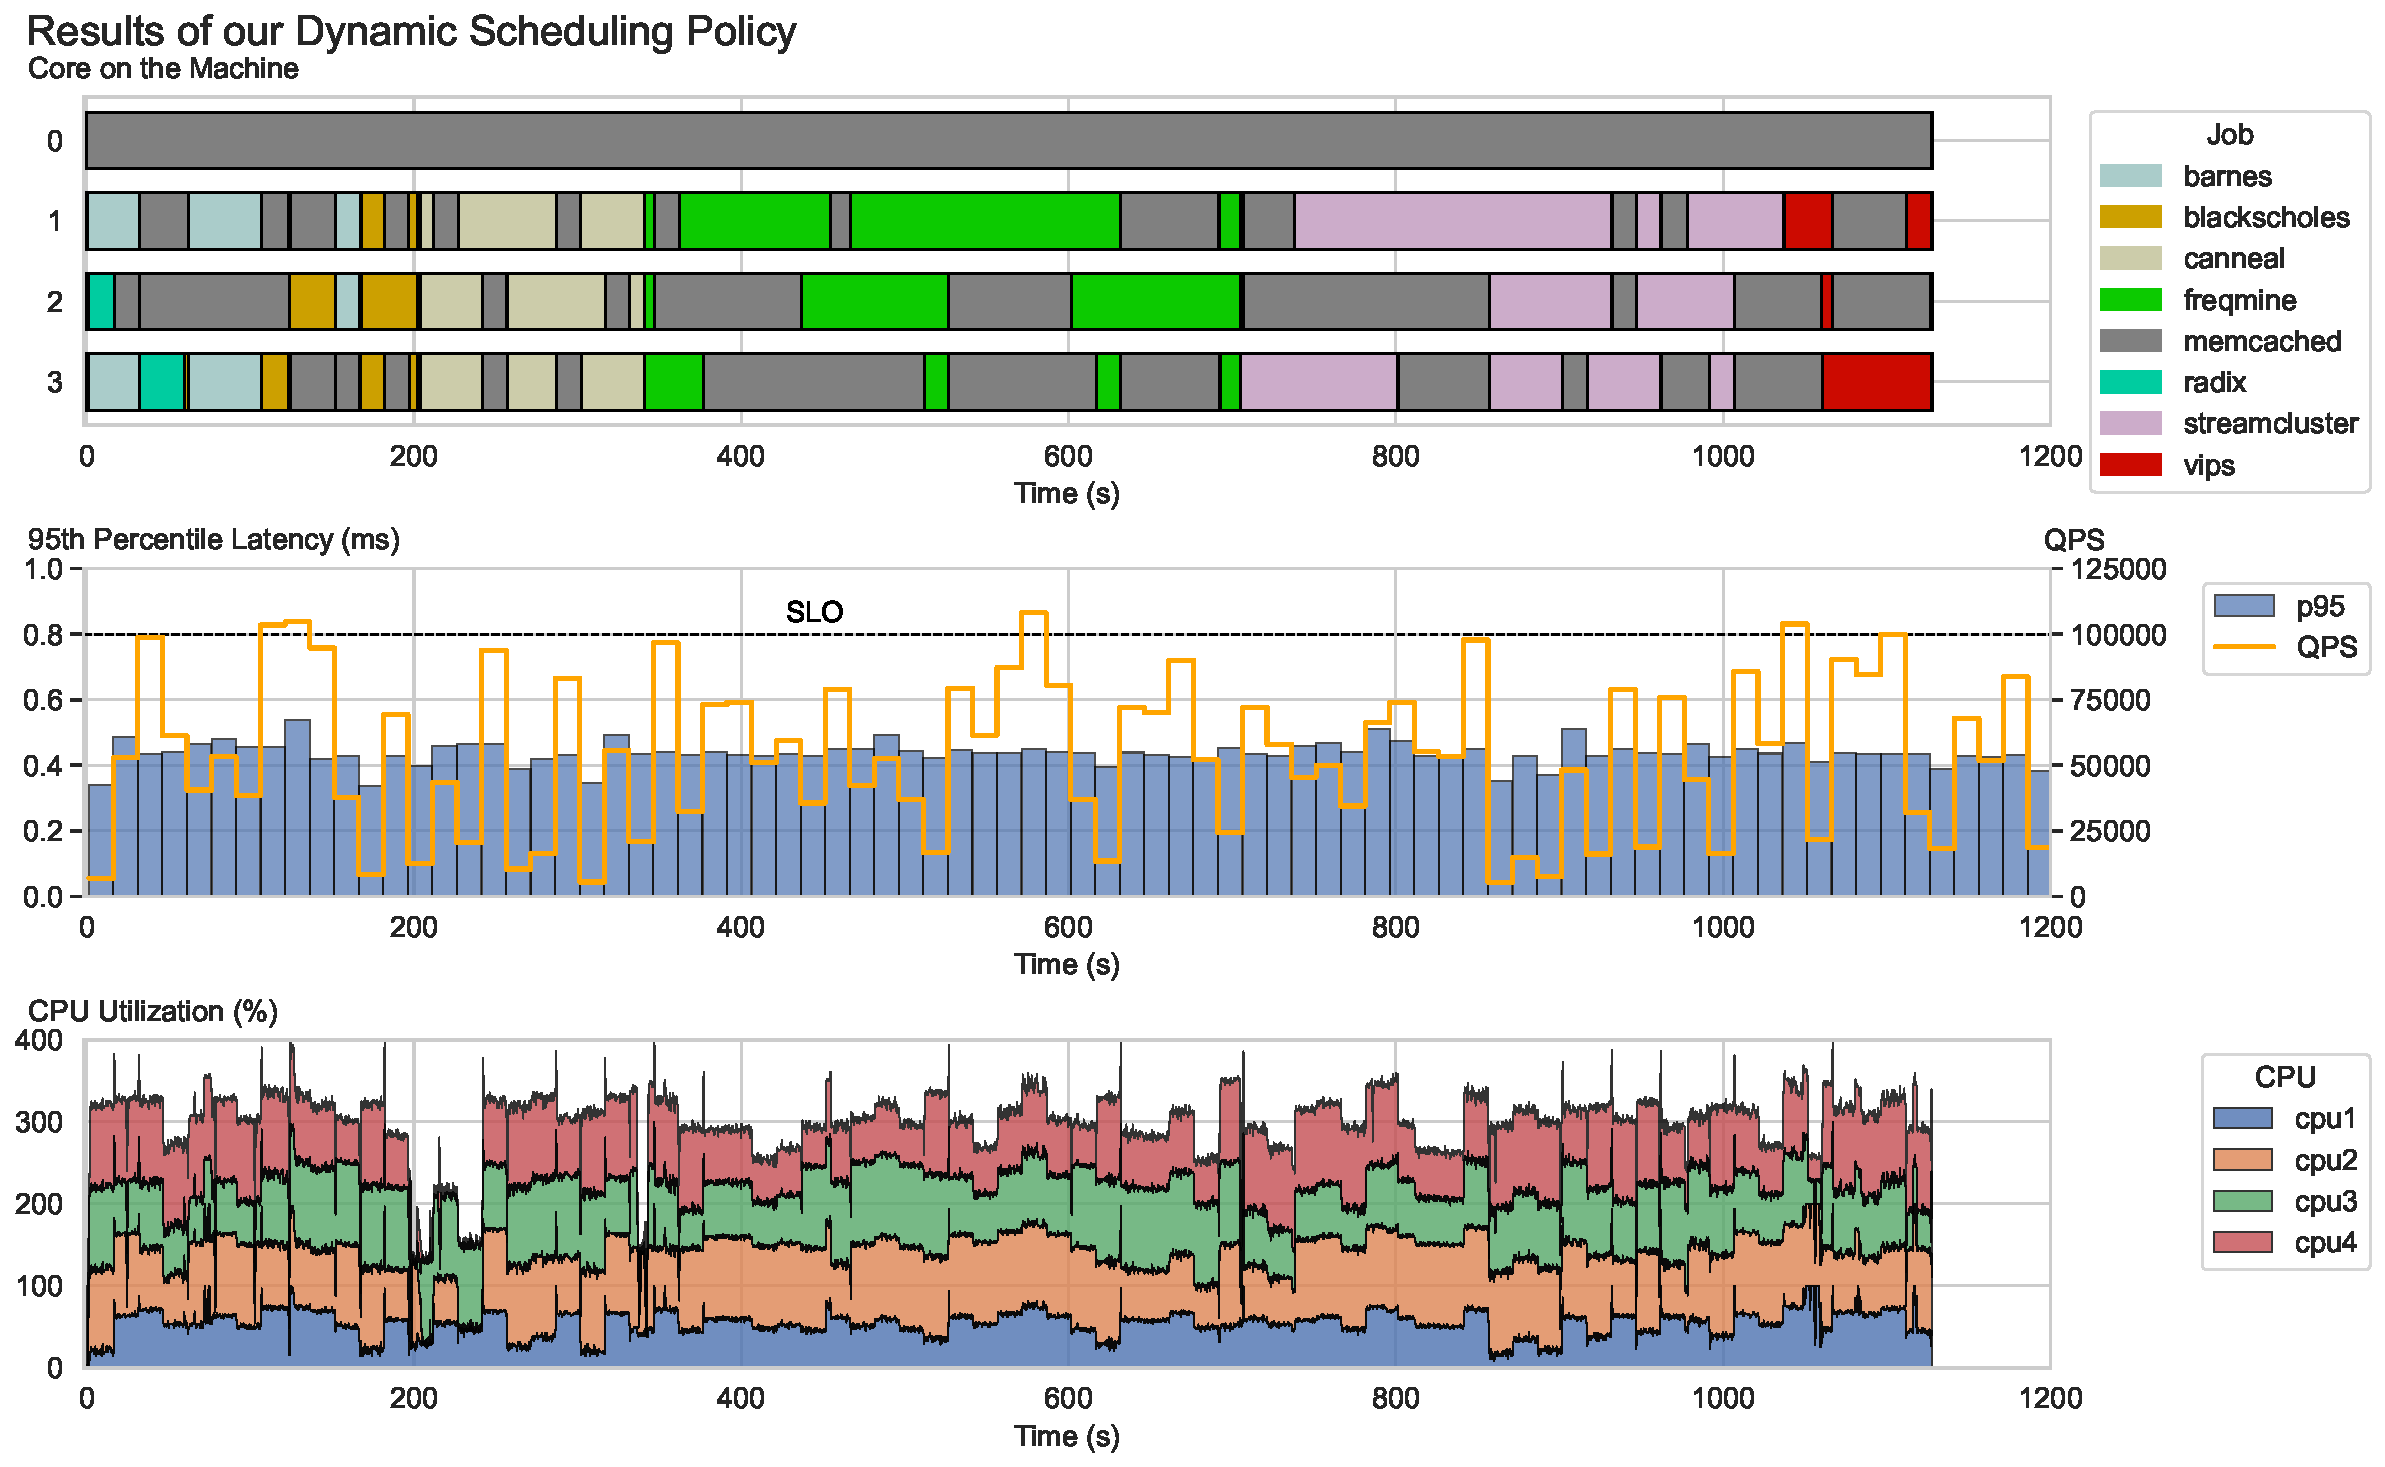
\includegraphics[width=1\linewidth]{report/figures/part4_q3_2.pdf}
       \caption{Second run of our dynamic scheduling policy, showing on the first plot the scheduling of the jobs over the cores over time, on the second plot the 95th percentile latency (blue bars) with the SLO of $0.8 ms$ as a black line, and achieved QPS (orange line) over time, and on the third plot the CPU utilization of the cores. Running all jobs took $\approx 1128$ seconds ($\approx 18.8$ minutes), and resulted in $0\%$ violations of the SLO.}
       \label{fig:part4_q3_2}
   \end{figure}

   \begin{figure}[H]
       \centering
       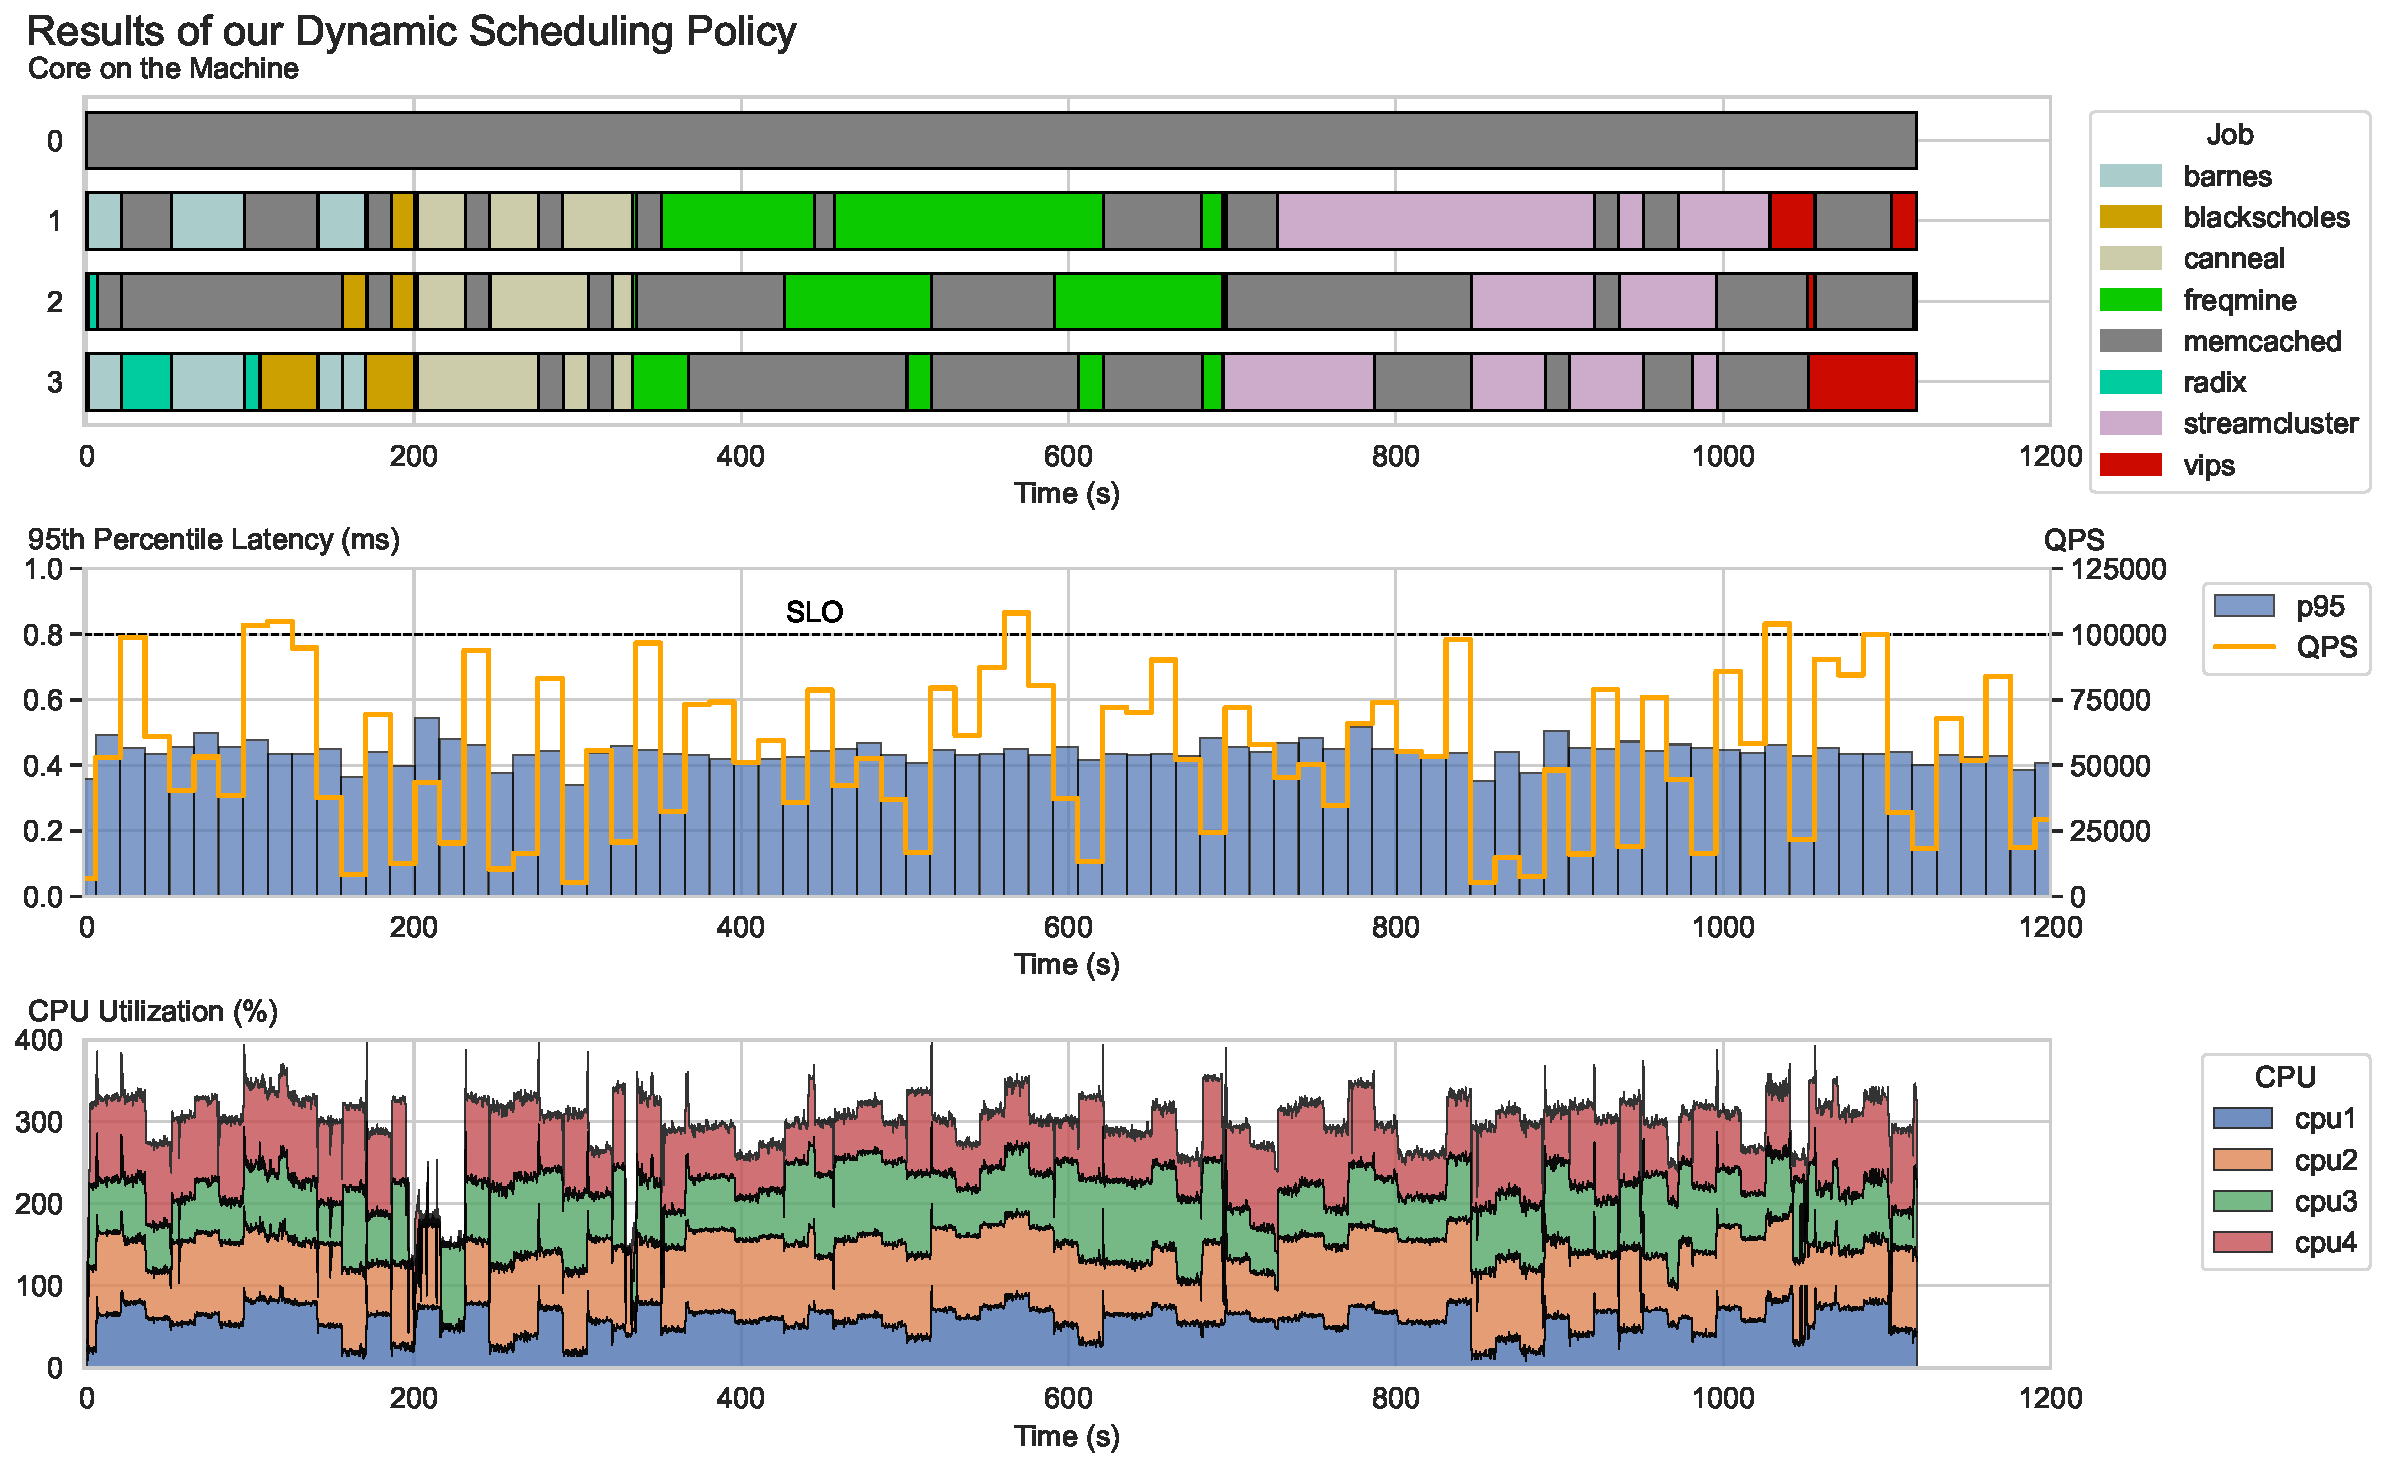
\includegraphics[width=1\linewidth]{report/figures/part4_q3_3.pdf}
       \caption{Third run of our dynamic scheduling policy, showing on the first plot the scheduling of the jobs over the cores over time, on the second plot the 95th percentile latency (blue bars) with the SLO of $0.8 ms$ as a black line, and achieved QPS (orange line) over time, and on the third plot the CPU utilization of the cores. Running all jobs took $\approx 1118$ seconds ($\approx 18.6$ minutes), and resulted in $0\%$ violations of the SLO.}
       \label{fig:part4_q3_3}
   \end{figure}

    \item \textbf{[16 points]} Repeat Part 4 Question 3 with a modified \texttt{mcperf} dynamic load trace with a 5 second time interval (\texttt{qps\_interval}) instead of 10 second time interval. Use the following command: 
    
\begin{Verbatim}[fontsize=\small]
$ ./mcperf -s INTERNAL_MEMCACHED_IP --loadonly 
$ ./mcperf -s INTERNAL_MEMCACHED_IP -a INTERNAL_AGENT_IP \ 
           --noload -T 8 -C 8 -D 4 -Q 1000 -c 8 -t 1800 \ 
           --qps_interval 5 --qps_min 5000 --qps_max 110000 \ 
           --qps_seed 2345
\end{Verbatim}
    
    You do not need to include the plots or table from Question 3 for the 5-second interval. Instead, summarize in 2-3 sentences how your policy performs with the smaller time interval (i.e., higher load variability) compared to the original load trace in Question 3. 

    \textbf{Summary:} % Place your summary here.
    \\
    
    What is the SLO violation ratio for memcached (i.e., the number of datapoints with 95th percentile latency $>$ 0.8ms, as a fraction of the total number of datapoints) with the 5-second time interval trace? The SLO violation ratio should be calculated during the time from when the first batch-job-container starts running to when the last batch-job-container stops running.

    \textbf{Answer:} % Place your solution here.
    \\
    
    What is the smallest \texttt{qps\_interval} you can use in the load trace that allows your controller to respond fast enough to keep the memcached SLO violation ratio under 3\%? 
    
    \textbf{Answer:} % Place your solution here.
    \\
    
    What is the reasoning behind this specific value? Explain which features of your controller affect the smallest \texttt{qps\_interval} interval you proposed.

    \textbf{Answer:} % Place your solution here.
    \\

    Use this \texttt{qps\_interval} in the command above and collect results for three runs and fill out the table below. %Include the same types of plots (1A, 1B, 2A, 2B, 3A, 3B) and table as in Question 3. 
    
    \begin{table}[ht]
        \centering
        \begin{tabular}{ |c|c|c|c|c|} 
            \hline
            job name & mean time [s] & std [s] \\ \hline \hline
            \coloredcell{barnes}           & & \\  \hline
            \coloredcell{blackscholes}     & & \\  \hline
            \coloredcell{canneal}          & & \\  \hline
            \coloredcell{freqmine}         & & \\  \hline
            \coloredcell{radix}            & & \\  \hline
            \coloredcell{streamcluster}    & & \\  \hline
            \coloredcell{vips}             & & \\  \hline
            total time      & & \\  \hline
        \end{tabular}
    \end{table}

    \textbf{Plots:} % Place your plots here.
\end{enumerate}

\noindent
\textbf{\underline{Use of AI Tools}: Did you use any AI tools for this project? If so, disclose them here and explain what you used the tool(s) for and why. Note that the use of AI tools is NOT needed and NOT expected for the project.} 